\subsection{Information-centric Networking}
\label{sec:netinf}
The Internet was originally designed based on a host-centric paradigm 
(one-to-one communication), where users explicitly connect to hosts 
in order to use services and retrieve resources. In the early days 
this worked well due to the low amount of users per host, but as the 
internet gained popularity the use of services began to increase. 
Over the past decades, the host-centric approach has become a 
growing impediment for services with large user bases, with workarounds 
like load-balancing and content delivery networks to circumvent 
bandwidth bottle necks in place. Today most traffic involves 
transferring of audio/video media and social networking content,
 both relying on one-to-many communication. Information-centric
 networking (ICN) is a research field aiming to redesign the internet
 in a fundamental way for today's and the near future's usage patterns. 
In ICN, the actual host providing a specific resource or service can
 be arbitrary and therefore unknown to the user. Instead of connecting 
to a host, the user queries the network as a whole. This enables 
low-level caching in every network node, so that repeated forwarding 
of identical information can be minimised and bandwidth can thus be used more
 efficiently. The main challenges in ICN are the ways of addressing 
information units and the integration with existing, host-centric networks. 
At this time ICN only exists in the form of independent research projects 
(e.g. NetInf), with no cross-industry standards on the horizon
 yet \cite{ICNarticle}. 


\subsection{Network of Information}
Network of Information (NetInf) was one of the first approaches proposed 
by the 4WARD project \cite{4ward}. This ICN paradigm was intended to deal 
with the issues that the current Host-Centric Networks suffer from. Every 
object on the network is called a Named Data Object (NDO) and is self-verifying.
 This leads to the user being able to request a certain object, an NDO, 
and fetch it from any source without worrying who or where it gets it from.
 The NDO can verify itself by using its own hash value as part of its name
 along with the used hash-algorithm.
A lot has changed in NetInf since the 4WARD project made the first draft. 
Currently the most recent versions are managed by the SAIL project \cite{sail}. Figures \ref{fig:ndorequest1} and \ref{fig:ndorequest2} show, at the conceptual level, two ways that NetInf can handle NDO requests.

\begin{figure}[H]
	\centering
		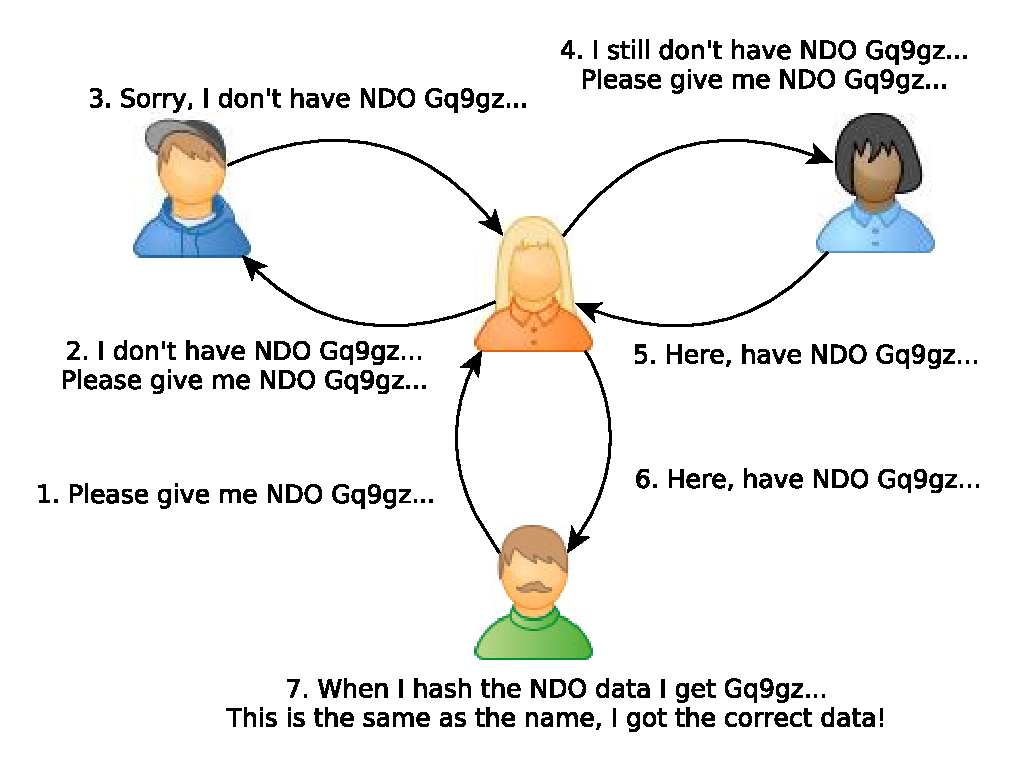
\includegraphics[width=1.00\textwidth, angle=0]{./img/netinf2.pdf}
    	\caption{Handling an NDO request using forwarding}
	\label{fig:ndorequest1}
\end{figure}

\begin{figure}[H]
	\centering
		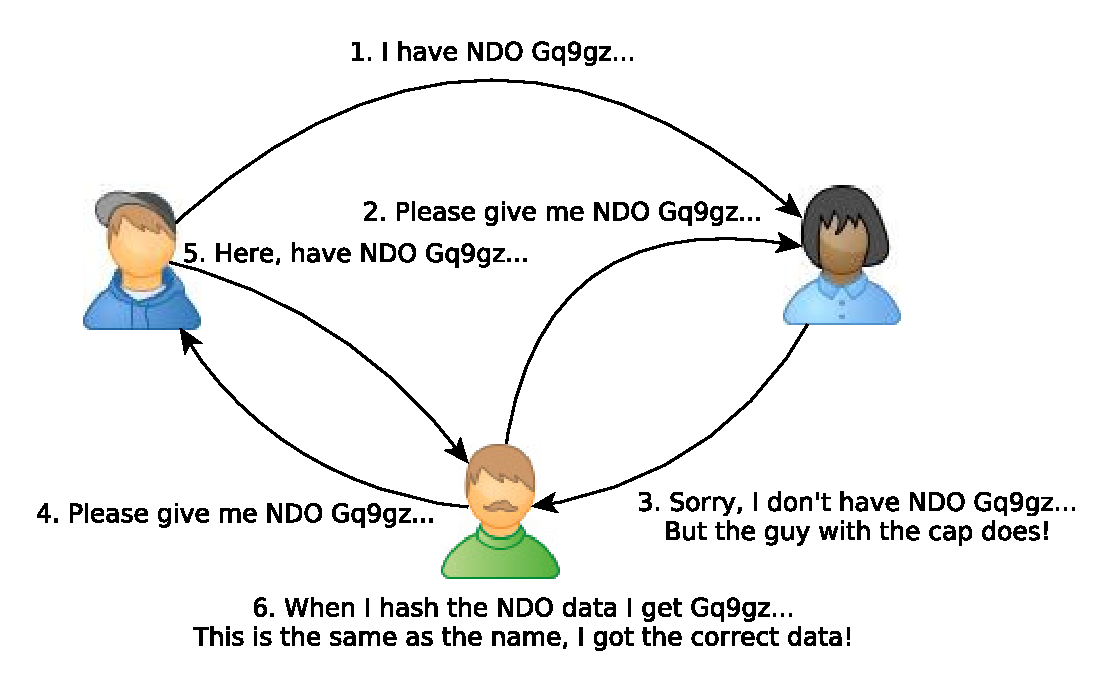
\includegraphics[width=1.00\textwidth, angle=0]{./img/netinf1.pdf}
    	\caption{Handling an NDO request using locators}
	\label{fig:ndorequest2}
\end{figure}

\subsection{OpenNetInf}
OpenNetInf \cite{opennetinf} is an open source Java implementation of NetInf
 developed at the University of Paderborn. OpenNetInf is still in the very
 early development phase and mainly aimed at research. The frontend development
 team decided to use OpenNetInf as a starting point for the Android client's
 NetInf functionality, but still had to implement and extend it to provide additional functionality. One reason for choosing OpenNetInf, rather than 
starting from scratch, was to avoid reinventing the wheel. It was also a 
chance to contribute to an existing project. Another reason was the closely
 related work done in a previous master thesis \cite{hugomiguel} which used 
OpenNetInf.
